% !TEX root =  main.tex
\eat{\section*{Notes}
\begin{itemize}
\item Are you pitching the resource or the technique? The answer is the technique. The pitch is essentially that of acquiring representations about any target resource by explicitly querying for easy to extract sentences. This works for certain types of target concepts.
\item Pitch broadly to any domain where the target phenomena are described in many ways. 
\item Pitch utility for other applications.
\item How is this different from relation extraction?
\item Acknowledge the focus is on sentences that contain the process name. Often times discourse is needed to extract other information.
\item What is the secret sauce? It is the sauce that was used for Open IE, ie., leveraging extractable sentences those which convey information in expected ways.
\item What is the formalism? Constrained Conditional Models or Graphical Models? 
\item Is there any issue with using Google API? Mention you will consider using ClueWeb or PeterT's corpus.
\item How is the work different from semi-supervised and unsupervised semantic role induction?
\item How is this different from template induction for event extraction? 
\end{itemize}
\newpage
}
\section{Introduction}
\eat{
Question answering and knowledge extraction research has focused on extracting and reasoning with simple facts expressible as binary relations.
Open-domain QA and factoid question answering on the web has driven much of this research. 
In contrast grade-level science exams go beyond retrieval abilities and test understanding and use of knowledge to reason about specific scenarios~\cite{clark2014:akbc}.

% in a form that is effective for reasoning a
% ability to recognize a scenario and map elements of the scenario to known scientific processes or phenomena. 
%We refer to this as process recognition.
%We propose automatic acquisition of semantic-role based knowledge base of simple physical, chemical, and other natural phenomena. 
% Our vision is to acquire knowledge that can be used to effectively reason about scenarios and situations using scientific knowledge.
}

Our vision is targeted acquisition of inference-supporting knowledge that can be used for reasoning tasks such as Question Answering (QA).
In particular we focus on knowledge acquisition for standardized test benchmarks such as grade-level science exams~\cite{clark2015elementary}.  Our prior work on these tasks provide strong motivation for reasoning based approaches~\cite{clark2014:akbc,chb2013:akbc}.
Lexical and syntactic variations render shallow text-derived knowledge ineffective for reasoning, even when using advanced state-of-the-art techniques~\cite{khot2015:emlnlp}. 
Deeper semantic representations are critical for effective reasoning.

This proposal investigates methods for acquiring knowledge about physical, chemical, and other natural phenomena.
The goal is to derive knowledge that allows effective reasoning about scenarios involving these phenomena. We refer to this as process knowledge. 
Our representation and acquisition methods will be targeted towards the grade science benchmarks but the methodology is general and can be applied to other tasks and domains.

\subsection{Motivation}
We motivate the need for a semantic-role based representation using two examples from 4$^{th}$ grade science exams. These questions test the ability to recognize a process based on the description of a scenario. \\

\begin{figure}[hbt]
	\begin{center}
	%9.06 x 4.35
	%12.08 x 2.9
	\vspace{-1em}
	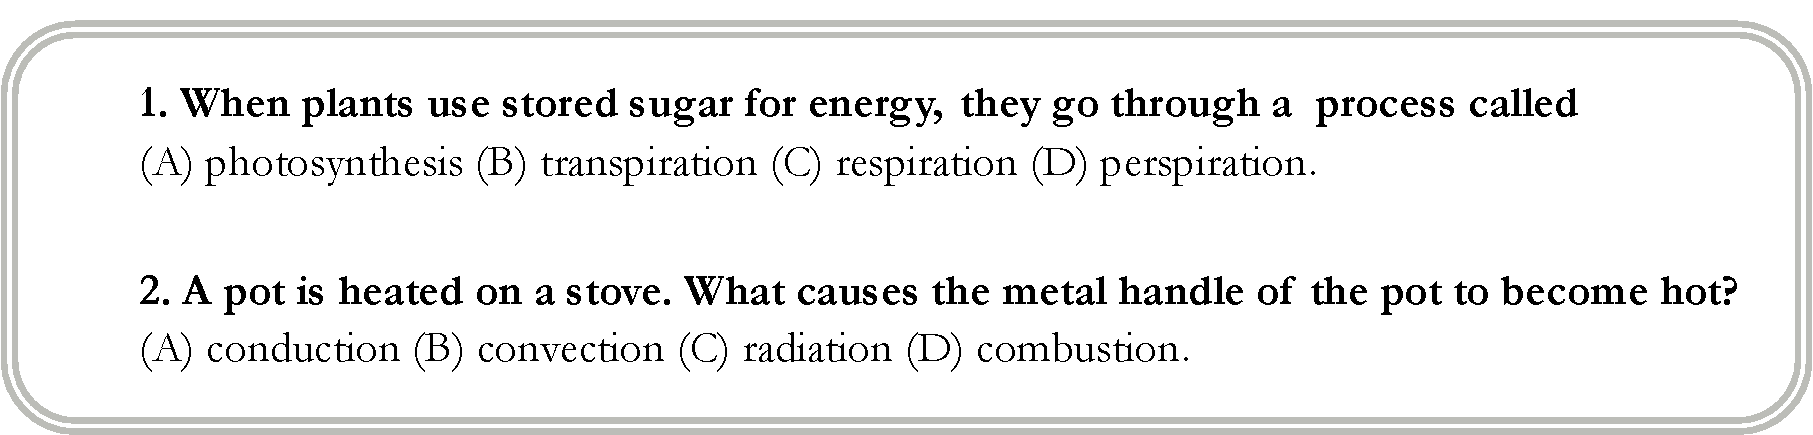
\includegraphics[width=6.04in,height=1.45in]{figures/questions-stretch.pdf} 	
	\caption{\label{fig:questions} {Example Questions from New York Regents Exam.}}
	\end{center}
\end{figure}

\eat{\begin{center}
\framebox{
\begin{minipage}{36em}
\begin{enumerate}
	\item {\em When plants use stored sugar for energy, they go through a process called\\
	(A) photosynthesis (B) transpiration (C) respiration (D) perspiration.}\\
	
	\item {\em A pot is heated on a stove. What causes the metal handle of the pot to become hot? \\
	(A) Conduction (B) Convection (C) Radiation (D) Combustion}. \\
\end{enumerate}

\end{minipage}

}
\\
\end{center}
}


%The knowledge necessary for this task is naturally expressed via simple semantic roles. 
The first question tests knowledge about biological processes.
{\em Photosynthesis} and {\em respiration} both involve sugar and energy. 
Photosynthesis converts light energy to sugar, whereas (cellular) respiration releases energy in the sugar by breaking it down. 
Not surprisingly these processes are described using similar words, which makes bag-of-words style reasoning unreliable. 
Understanding the different roles that energy and sugar play in these processes, and knowledge of the main actions involved is key to effective reasoning.

The second question tests knowledge about heat transfer mechanisms.
To establish that conduction is the cause, a reasoning system must establish that there is some heat transfer happening through {\em direct contact}. 
We envision a reasoning system that first interprets the input scenario in terms of entities and their semantic roles. 
In this case, the system would first identify {\em what is being heated} (the pot), and {\em what is the purported result} of the heating (the pot handle). 
Then, it will verify if this interpretation of the actions and the roles match with the expected actions and roles of a conduction process. 
Specifically the knowledge about conduction should convey that there are two entities that are in direct contact, one of which is being heated or is hot, 
and the result of conduction is that the other object also becomes {\em hot}. 
These bits of information are naturally encoded as semantic roles.

Existing lexical semantic resources and knowledge bases are not well suited for our goals.

On the one hand, existing semantic resources such as FrameNet and PropBank provide different representations of 
general open-domain actions but do not cover knowledge about scientific processes. 
FrameNet, for instance, does not have entries for nearly half of the processes described in 4th grade science exams. 
The coverage is likely worse for higher grade levels. 
On the other hand, automatic knowledge bases built via relation extraction
capabilities (e.g., Open IE) scale to arbitrary target concepts but only contain simple binary relations e.g., (Arg1, Rel, Arg2), that do not adequately capture the semantics.

\subsection{Proposal}

In response, we propose to build a knowledge base about physical, chemical, and biological processes from their textual descriptions. 
\todo{Add a figure that shows a snippet from the KB we expect to produce.}
%While there has been much work in linguistics on identifying a complete list of thematic roles~\cite{}, there is not much of a consensus~\cite{}.
%ProbBank style role labeling largely focused on a predicate centric view, which is appropriate for reasoning about general purpose actions (e.g., change, get, give). 
%Our goal is to construct process level abstractions to reduce burden during reasoning, which is closer to a FrameNet style abstraction.
%Pre-specifying frames requires expert labor and is not scalable.

\subsubsection*{Representation}
We compose a semantic representation using a combination of pre-determined vocabulary of semantic roles and derive new roles on demand.
{\bf We propose to identify roles with respect to a canonical version of the process, rather than based on the actual lexical realization in the sentence.}
This is similar to frame centric abstraction used by FrameNet. The key difference is that roles are still thematic but are defined with respect to a canonical predicate.
Canonicalization during construction reduces reasoning burden by eliminating steps that only serve to establish equivalence of information realized via different predicates.

%General semantic role labeling task is challenging because of the lexical and syntactic variations in role realizations. 
\subsubsection*{Role Extraction and Joint Inference}

Handling the variations requires learning from large amounts of training data, which is laborious and requires expert labor.
Also mentioned above, existing resources cannot be directly used. FrameNet does not cover the concepts of interest. 
The need for a canonicalized representation precludes the direct use of existing annotations or tools built for PropBank.
Rather than building a role labeler that can work on any sentence, we adopt a simpler approach that works well on a smaller subset of sentences.

{\bf The main idea is a targeted acquisition of knowledge from sentences that convey information in expected ways.}
Leveraging the vastness of the web greatly reduces the need to accurately identify roles in difficult to process sentences.
Using a set of manually constructed query patterns we find sentences which convey the roles using expected lexico-syntactic constructs. 
For instance "<process name> causes <x>" is a simple pattern that can be used to find the {\em result} role for a process. 
This strong expectation for how arguments are realized allows us to turn SRL into a simpler task of assessing the confidence on the extraction using features that generalize better across different processes.  
This allows us to substantially reduces the burden of annotating sentences for each process.
Even though PropBank and FrameNet data are not directly usable, the predicate-based roles and the frame structures can provide evidence for composing our target semantic roles. 
We propose to exploit these features to build a local sentence-level extractor.


Despite the targeted acquisition, local sentence-level extraction alone is not adequate, because not all lexico-syntactic patterns are unambiguous. 
For example, "evaporates into <x>" extracts steam, a {\em result}, as well as atmosphere, a {\em location}. 

{\bf A second key idea is to perform joint inference over multiple sentences to avoid errors in the local extraction}.
Because our goal is to acquire knowledge about a process, we turn the variety of expression on the web to our advantage. 
We build on prior work in Integer Linear Program (ILP) based semi-supervised and unsupervised induction approaches. 
The ILP attempts to find an assignment of roles that maximizes the sum of extraction confidences, 
while also minimizing disagreements in labels for similar text spans in similar sentences.

\subsubsection*{Assessment and Discovery}
While we start with a set of general purpose roles, {\em a priori} we don't assume which roles are applicable to each process as this manual assignment is not desirable from a scalability standpoint.
Also not all critical information may be covered by the set of roles that hand.

{\bf A third contribution of this proposal includes methods that identify the subset of roles that apply to a process and discover new roles not part of the general vocabulary}. 
As part of the targeted acquisition, we propose an iterative approach with methods to i) assess the coverage of the roles, ii) induce new roles by identifying consistently repeated arguments that don't fit existing roles, and iii) relevance feedback based query pattern generation to expand the knowledge.

\subsubsection*{Evaluation}

The generated knowledge base will be evaluated for intrinsic quality and external utility. For internal evaluations we will perform manual evaluation of the resulting KB. As part of the evaluation, {\bf we will also create a large scale curated KB, which relies on correcting the outputs from the system, rather than careful annotation of each sentence}. We will also generate a gold standard of the desired roles and role fillers for evaluating coverage. As an external evaluation we will use the knowledge base for answering process recognition questions. All the resources and evaluation test beds will be shared with the research community for further research.

\subsection{Prior Work and Contributions}

The motivation and direction for this proposal stems directly from our prior work on grade science exams.  Our earlier work studied knowledge requirements~\cite{chb2013:akbc}, developed inference-supporting rule knowledge bases~\cite{clark2014:akbc}, and investigated sophisticated state-of-the-art probabilistic reasoning methods for QA~\cite{khot2015:emlnlp}. Our ongoing preliminary work investigated the value of a handful of semantic roles in answering process recognition questions and identified the knowledge, representation, and reasoning gaps~\cite{louvan2015:kcap}. This proposal aims to address the central challenges that we've identified through these prior works.

Upon successful completion this project would have made the following contributions:
\begin{itemize}
\item Release of a knowledge base covering semantic representations of processes for grade level science.
\item Methods for gathering high quality sentences that cover a target set of roles. 
\item A joint inference method that reconciles roles across different sentences.  
\item Methods for assessing applicability, coverage and discovery of new roles.
\end{itemize}



